\subsection[Graham]{Graham Scan}

\begin{frame}
\frametitle{Graham Scan}
Method of computing the convex hull of a finite set of points in the plane with time complexity O(n log(n)). The algorithm finds all vertices of the convex hull ordered along its boundary.
\end{frame}

\begin{frame}
\frametitle{Graham Scan}
\framesubtitle{Idea}
\begin{itemize}
\item find the point with the lowest y-coordinate. if there are multiple points with the lowest y-coordinate, the pick that one of them with the lowest x-coordinate. call this point P
\item now sort all the points in increasing order of the angle they and point P make with the x-axis
\item consider each point in the sorted array in sequence. For each point determine whether coming from the 2 previous points it makes a left of a right turn.
\item if it makes a left turn, proceed with the next point
\item if it makes a right turn, the second-to-last point is not part of the convex hull and should be removed from the convex hull, continue this removing for as long as the last 3 points make up a right turn 
\end{itemize}
\end{frame}

\begin{frame}
\frametitle{Graham Scan}
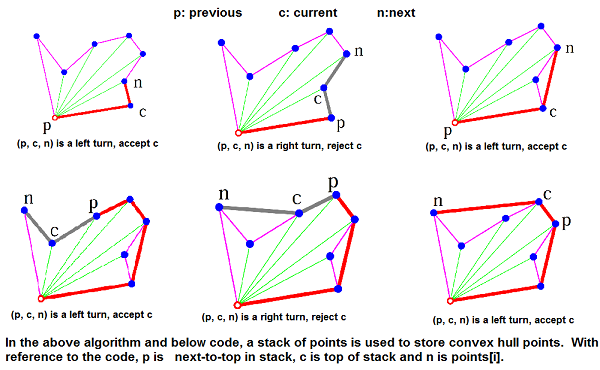
\includegraphics[width=1\textwidth]{./2-convex/img/graham}
\end{frame}

\begin{frame}
\frametitle{Graham Scan}
\framesubtitle{Direction of the turn}
To determine whether 3 points constitute a left or a right turn we do not have to compute the actual angles but we can use a cross product.\\
Consider the 3 points $(x_{1}, y_{1})$,  $(x_{2}, y_{2})$ and $(x_{3}, y_{3})$, which we will call $P_{1}, P_{2}$ and $P_{3}$.\\
Now compute the z-component of the cross product of the vectors $P_{1}P_{2}$ and $P_{1}P_{3}$. Which is given by the expression $(x_{2}-x_{1})(y_{3}-y_{1})-(y_{2}-y_{1})(x_{3}-x_{1})$.\\
If the result is 0, the points are collinear. If the result is positive, the 3 points constitute a left turn. If the result is negative, the 3 points constitute a right turn.
\end{frame}